\documentclass[a4paper,12pt]{article}
\usepackage{fontspec}
\usepackage[croatian]{babel}
\usepackage{graphicx}
\usepackage{hyperref}
\usepackage{geometry}
\usepackage{setspace}   
\usepackage{enumitem}
\usepackage{listings}
\usepackage{xcolor}
\usepackage{multicol}
\setmainfont{Times New Roman}
\geometry{a4paper, margin=2.5cm}
\doublespacing
\setlength{\parindent}{1.5cm}

\lstdefinestyle{sqlstyle}{
    language=SQL,
    basicstyle=\small\ttfamily,
    numbers=left,
    numberstyle=\tiny,
    numbersep=5pt,
    frame=single,
    breaklines=true,
    breakatwhitespace=true,
    showstringspaces=false,
    tabsize=2,
    keywordstyle=\color{blue},
    stringstyle=\color{red},
    commentstyle=\color{green!60!black},
}

\begin{document}

\begin{center}
    
\includegraphics[width=0.3\textwidth]{edunova_logo.png}
\end{center}

\begin{center}
    {\Large Program obrazovanja za stjecanje mikrokvalifikacije web programiranje}\\[2ex]
    GRUPA WP7\\[2ex]
    \vspace{10em}
    {\Huge \textbf{Dokumentacija završne provjere}}\\[2ex]

\end{center}

\begin{center}
    \vspace{2em}
    {\Large {Platforma za organizaciju rada (ZORA)}}\\[2ex]
\end{center}

\begin{center}
    \vspace{2em}
    \noindent\textbf{git URL aplikacije:} \url{https://github.com/tnebes/zora}\\[1ex]
    \textbf{URL produkcije:} \url{https://zora.draucode.com}
\end{center}

\vspace{2cm}

\begin{center}
    \noindent{\Huge{\textbf{Tomislav Nebes}}}
\end{center}

\vfill
\begin{center}
    {\large Osijek, ožujak 2025.}
\end{center}

\newpage

\tableofcontents
\newpage

\section{Uvod}

Platforma za organizaciju rada, nadalje ZORA, je web aplikacija koja omogućava organizaciju i planiranje posla općenito. Ona omogućava korisnicima da dodaju zadatke koje kasnije na temelju informacija dostupnih u zadaćama (\emph{eng. tasks}) mogu biti obavljeni. Motivacija za kreiranje ZORE je postojanje Adobe proizvoda naziva Workfront koji je također alat za organizaciju posla, s time da posjeduje značajno više funkcionalnosti nego što ZORA trenutno ima.

Glavne funkcionalnosti ZORE uključuju kreiranje zadataka, dodjeljivanje zadataka korisnicima, praćenje napretka zadataka te generiranje prikaza stanja zadataka. Aplikacija bi posebno bila korisna za timove koji rade na projektima i trebaju organizirati svoje zadatke i rokove.

Iz tehnološke perspektive, ZORA je izgrađena pomoću platforme ASP.NET Core 9.0 s korištenjem Entity Framework (EF) Core za komunikaciju s bazom podataka Microsoft SQL Server. Korisničko sučelje je izgrađeno pomoću HTML, CSS i TypeScript. Dakle, \emph{eng. frontend} je izgrađen pomoću Angular razvojnog okvira (eng. framework), a \emph{eng. backend} pomoću ASP.NET Core.

ZORA ima za cilj omogućiti jednostavno i efikasno upravljanje zadacima, s mogućnošću prilagodbe za različite veličine timova i projekata. Planovi za daljnji razvoj uključuju implementaciju novih značajki poput integracije s drugim alatima, povezivanja zadataka s projektima, naprednih alata za praćenje napretka te optimizacije za mobilne uređaje. S tehničke strane, prioriteti su unapređenje performansi, modernizacija korisničkog sučelja i poboljšanje mobilne kompatibilnosti.

\section{Vježbe}

Rad na ZORA aplikaciji se vršio postepeno tijekom cijelog edukacijskog smjera. Vježbe su se odnosile na razvoj ERA dijagrama, \emph{backend} aplikacije te \emph{frontend} aplikacije. U sljedećim poglavljima će biti opisane vježbe i njihov rezultati.

\subsection{ERA dijagram (Vježba 1)}

Cilj prve vježbe je bio napisati \emph{Structured Query Language}, nadalje SQL, skriptu koja je omogućila kreiranje baze podataka. U svrhu provjere ispravnosti skripte je korišten Microsoft SQL Server Management Studio (SSMS) pomoću kojeg je izvršena vizualna provjera kreirane baze podataka kao i unos testnih podataka u tablice.

Baza podataka je kreirana u dvije faze. Prva faza uključuje inicijalnu postavku baze podataka i korisničkih dozvola:

\begin{lstlisting}[style=sqlstyle]
CREATE DATABASE zora;
ALTER DATABASE zora COLLATE Latin1_General_100_CI_AS_SC_UTF8;
CREATE LOGIN [zora_service] WITH PASSWORD = 'your_strong_password_here';
CREATE USER [zora_service] FOR LOGIN [zora_service];
\end{lstlisting}

Druga faza uključuje kreiranje tablica i relacija. Glavne tablice uključuju:

\begin{itemize}
    \item \texttt{zora\_users} - pohranjuje podatke o korisnicima
    \item \texttt{zora\_roles} - definira uloge u sustavu
    \item \texttt{zora\_work\_items} - centralna tablica za upravljanje zadacima
    \item \texttt{zora\_projects} i \texttt{zora\_tasks} - specifične vrste radnih stavki
\end{itemize}

Primjer kreiranja tablice za korisnike:

\begin{lstlisting}[style=sqlstyle]
CREATE TABLE zora_users (
    id BIGINT IDENTITY(1,1) PRIMARY KEY,
    username VARCHAR(255) NOT NULL,
    password VARCHAR(255) NOT NULL,
    email VARCHAR(255) NOT NULL,
    created_at DATETIME2 DEFAULT GETDATE(),
    deleted BIT DEFAULT 0 NOT NULL,
    CONSTRAINT CHK_User_Email CHECK (email LIKE '%_@__%.__%')
);
\end{lstlisting}

Baza podataka implementira soft delete mehanizam kroz \texttt{deleted} zastavicu u većini tablica. Relacije između tablica su definirane kroz vanjske ključeve, što osigurava referencijalni integritet podataka. Primjer relacije između korisnika i uloga:

\begin{lstlisting}[style=sqlstyle]
CREATE TABLE zora_user_roles (
    user_id BIGINT NOT NULL,
    role_id BIGINT NOT NULL,
    PRIMARY KEY (user_id, role_id),
    FOREIGN KEY (user_id) REFERENCES zora_users(id),
    FOREIGN KEY (role_id) REFERENCES zora_roles(id)
);
\end{lstlisting}

Nakon kreiranja strukture, dodani su početni podaci, uključujući administratorskog korisnika i osnovne uloge:

\begin{lstlisting}[style=sqlstyle]
INSERT INTO zora_users (username, password, email) 
VALUES ('tnebes', '$2a$12$u8XHrlyC7Y1X96jTawebd.Li3uK9Z.PImu6Vy9KD.rtMNnmz3SKY.', 
        'tnebes@draucode.com');
INSERT INTO zora_roles (name) VALUES ('Admin');
\end{lstlisting}

Baza podataka je optimizirana kroz indekse i ograničenja, što osigurava brz pristup podacima i valjanost unosa. Primjer optimizacije kroz indekse:

\begin{lstlisting}[style=sqlstyle]
CREATE UNIQUE INDEX IX_User_Username ON zora_users(username) WHERE deleted = 0;
CREATE UNIQUE INDEX IX_User_Email ON zora_users(email) WHERE deleted = 0;
\end{lstlisting}

Ova implementacija omogućava skalabilnu i sigurnu pohranu podataka za ZORA aplikaciju, s mogućnošću daljnjeg proširenja i optimizacije.

\begin{center}
    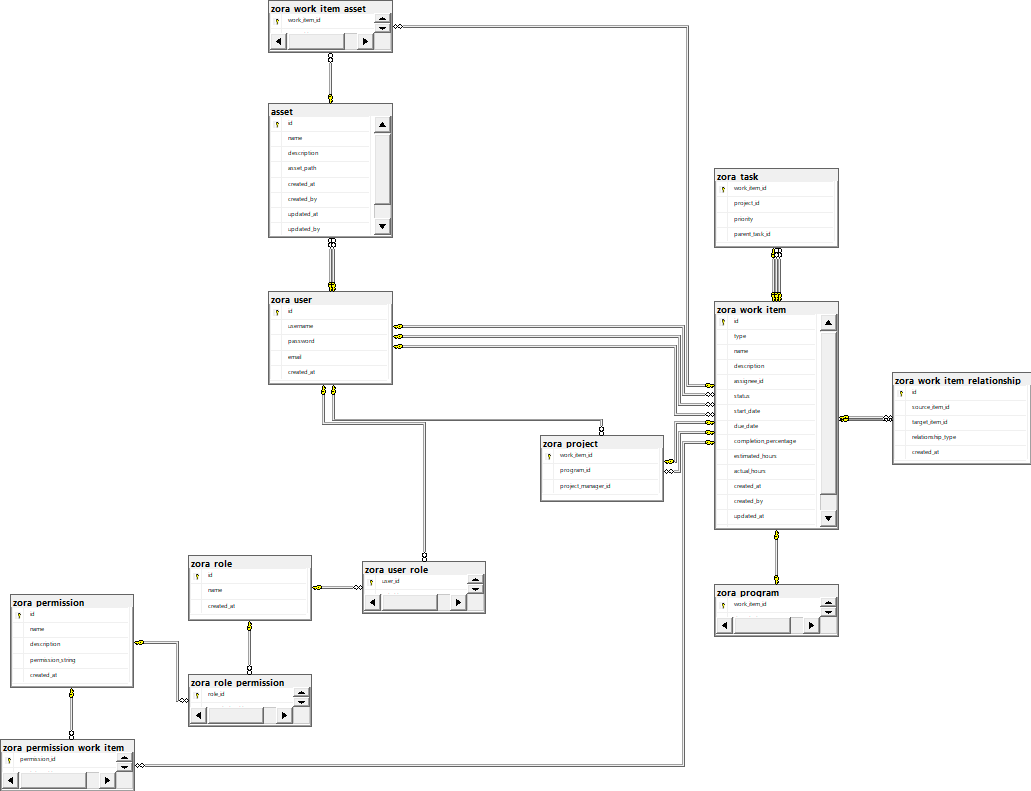
\includegraphics[width=\textwidth]{../zora_diagram.png}
\end{center}

ERA dijagram prikazuje strukturu baze podataka ZORA aplikacije. Svaka tablica ima svoje specifične atribute i relacije s drugim tablicama:

\begin{itemize}
    \item \textbf{zora\_users} sadrži osnovne podatke o korisnicima sustava:
        \begin{itemize}
            \item jedinstveni identifikator, korisničko ime, lozinku i email
            \item vremenske oznake kreiranja i soft-delete zastavicu
            \item povezuje se s ulogama kroz \texttt{zora\_user\_roles}
        \end{itemize}
    
    \item \textbf{zora\_roles} i \textbf{zora\_permissions} definiraju sigurnosni model:
        \begin{itemize}
            \item uloge (\texttt{roles}) definiraju skupine korisnika
            \item dozvole (\texttt{permissions}) koriste 5-bitni string za definiranje prava\footnote{Sustav dozvola koristi 5-bitni string gdje svaka pozicija predstavlja određenu razinu pristupa: \texttt{00000} (None), \texttt{00001} (Read), \texttt{00010} (Write), \texttt{00100} (Create), \texttt{01000} (Delete), \texttt{10000} (Admin). Na primjer, korisnik s dozvolom \texttt{00101} ima prava čitanja i kreiranja. Implementirano kroz \texttt{PermissionFlag} enum u C\# kodu gdje su dozvole definirane kao bitwise flags: None = 0, Read = 1, Write = 2, Create = 4, Delete = 8, Admin = 16.}
            \item veza many-to-many između uloga i dozvola kroz \texttt{zora\_role\_permissions}
        \end{itemize}
    
    \item \textbf{zora\_work\_items} je centralna tablica sustava:
        \begin{itemize}
            \item sadrži zajedničke atribute za sve vrste radnih stavki
            \item prati status, napredak, procijenjene i stvarne sate rada
            \item povezuje se s korisnikom kojem je zadatak dodijeljen (\texttt{assignee\_id})
            \item prati tko je kreirao i ažurirao stavku (\texttt{created\_by}, \texttt{updated\_by})
        \end{itemize}
    
    \item \textbf{zora\_programs}, \textbf{zora\_projects} i \textbf{zora\_tasks} definiraju planiranu hijerarhijsku strukturu\footnote{Hijerarhijska struktura programa i projekata je dio planiranog proširenja sustava. Trenutna implementacija podržava osnovne zadatke, dok će buduća nadogradnja omogućiti potpunu hijerarhijsku organizaciju rada.}:
        \begin{itemize}
            \item programi će moći sadržavati više projekata, omogućavajući grupiranje povezanih projekata
            \item projekti će pripadati programu i imati definiranog voditelja projekta
            \item zadaci su trenutno implementirani kao osnovne radne jedinice, s planiranom podrškom za hijerarhijsku organizaciju
        \end{itemize}
    
    \item \textbf{zora\_work\_item\_relationships} omogućava fleksibilno povezivanje:
        \begin{itemize}
            \item definira veze između različitih radnih stavki
            \item svaka veza ima svoj tip i vremenske oznake
            \item omogućava praćenje zavisnosti između zadataka
        \end{itemize}
    
    \item \textbf{assets} i \textbf{zora\_work\_item\_assets}:
        \begin{itemize}
            \item pohranjuju podatke o datotekama i resursima
            \item omogućavaju povezivanje resursa s radnim stavkama
            \item prate metapodatke o resursima i njihovim izmjenama
        \end{itemize}
\end{itemize}

Sve tablice implementiraju \texttt{soft-delete} mehanizam kroz \texttt{deleted} zastavicu, što omogućava očuvanje povijesti podataka. Vremenske oznake (\texttt{created\_at}, \texttt{updated\_at}) i reference na korisnike koji su izvršili promjene osiguravaju mogućnost praćenja promjena u sustavu. Indeksi su postavljeni na ključne stupce koji se često koriste u pretraživanju, što optimizira performanse upita.

\newpage

\subsection{Backend (Vježba 2)}

Backend aplikacije je implementiran kao REST API koristeći ASP.NET Core 9.0. API je organiziran u nekoliko glavnih područja koja pokrivaju različite funkcionalnosti sustava.

\subsubsection{Opis API-ja}

U ovome poglavlju će biti opisan API za backend aplikaciju. Za svaku funkcionalnost je definiran odgovarajući HTTP endpoint i njegova svojstva. U nastavku slijede sve funkcionalnosti koje API podržava, grupirane po sličnosti:

\begin{itemize}
    \item \textbf{Autentifikacija i Autorizacija}:
        \begin{itemize}
            \item \texttt{/api/v1/authentication/token} - generira JWT token za prijavljenog korisnika
            \item \texttt{/api/v1/authentication/check} - provjerava valjanost postojećeg tokena
            \item \texttt{/api/v1/authentication/current-user} - dohvaća podatke trenutnog korisnika
            \item \texttt{/api/v1/authorisation/is-authorised} - provjerava ima li korisnik određenu dozvolu
            \item \texttt{/api/v1/authorisation/is-admin} - provjerava je li korisnik administrator
        \end{itemize}
    
    \item \textbf{Upravljanje Zadacima}:
        \begin{itemize}
            \item \texttt{GET /api/v1/tasks} - dohvaća listu zadataka s paginacijom
            \item \texttt{POST /api/v1/tasks} - kreira novi zadatak
            \item \texttt{PUT /api/v1/tasks/\{id\}} - ažurira postojeći zadatak
            \item \texttt{DELETE /api/v1/tasks/\{id\}} - briše zadatak (soft delete)
            \item \texttt{POST /api/v1/tasks/\{id\}/assign} - dodjeljuje zadatak korisniku
            \item \texttt{POST /api/v1/tasks/\{id\}/complete} - označava zadatak kao završen
            \item \texttt{GET /api/v1/tasks/find} - napredno pretraživanje zadataka po više kriterija
            \item \texttt{GET /api/v1/tasks/search} - brzo pretraživanje zadataka po ključnoj riječi
            \item \texttt{GET /api/v1/tasks/priority/\{userId\}} - dohvaća prioritetne zadatke korisnika
            \item \texttt{GET /api/v1/tasks/\{id\}/assets} - dohvaća resurse povezane sa zadatkom
        \end{itemize}
    
    \item \textbf{Upravljanje Korisnicima}:
        \begin{itemize}
            \item \texttt{GET /api/v1/users} - dohvaća listu korisnika s paginacijom
            \item \texttt{POST /api/v1/users} - kreira novog korisnika
            \item \texttt{PUT /api/v1/users/\{id\}} - ažurira podatke postojećeg korisnika
            \item \texttt{DELETE /api/v1/users/\{id\}} - deaktivira korisnika (soft delete)
            \item \texttt{GET /api/v1/users/search} - brzo pretraživanje korisnika po ključnoj riječi
            \item \texttt{GET /api/v1/users/find} - napredno pretraživanje korisnika po više kriterija
        \end{itemize}

    \item \textbf{Upravljanje Ulogama i Dozvolama}:
        \begin{itemize}
            \item \texttt{GET /api/v1/roles} - dohvaća sve dostupne uloge
            \item \texttt{POST /api/v1/roles} - kreira novu ulogu
            \item \texttt{GET /api/v1/roles/search} - brzo pretraživanje uloga po nazivu
            \item \texttt{GET /api/v1/roles/find} - napredno pretraživanje uloga po kriterijima
            \item \texttt{GET /api/v1/permissions} - dohvaća sve dostupne dozvole
            \item \texttt{POST /api/v1/permissions} - kreira novu dozvolu
            \item \texttt{GET /api/v1/permissions/search} - brzo pretraživanje dozvola po nazivu
            \item \texttt{GET /api/v1/permissions/find} - napredno pretraživanje dozvola
        \end{itemize}
    
    \item \textbf{Upravljanje Resursima}:
        \begin{itemize}
            \item \texttt{GET /api/v1/assets} - dohvaća listu resursa s paginacijom
            \item \texttt{POST /api/v1/assets} - učitava novi resurs
            \item \texttt{PUT /api/v1/assets/\{id\}} - ažurira metapodatke resursa
            \item \texttt{DELETE /api/v1/assets/\{id\}} - briše resurs (soft delete)
            \item \texttt{GET /api/v1/assets/\{id\}/download} - preuzima resurs
            \item \texttt{GET /api/v1/assets/\{id\}/preview} - dohvaća pregled resursa
            \item \texttt{GET /api/v1/assets/search} - brzo pretraživanje resursa po nazivu
            \item \texttt{GET /api/v1/assets/find} - napredno pretraživanje resursa po kriterijima
        \end{itemize}
    
    \item \textbf{Pomoćne Funkcionalnosti}:
        \begin{itemize}
            \item \texttt{GET /api/v1/seed} - inicijalizira bazu podataka s testnim podacima (samo za razvoj)
        \end{itemize}
\end{itemize}

\noindent\textbf{Kratak opis ruta:}

\begin{multicols}{2}
\begin{itemize}
    \item \texttt{/authentication/*} - autentifikacija korisnika i upravljanje sesijama
    \item \texttt{/tasks/*} - CRUD operacije nad zadacima, uključujući pretraživanje i filtriranje
    \item \texttt{/users/*} - upravljanje korisničkim računima i profilima
    \item \texttt{/roles/*} - definiranje i upravljanje korisničkim ulogama
    \item \texttt{/permissions/*} - upravljanje dozvolama i pravima pristupa
    \item \texttt{/assets/*} - upravljanje datotekama i resursima
    \item \texttt{/seed} - inicijalizacija testnih podataka (samo razvoj)
\end{itemize}
\end{multicols}

\subsubsection{Dodatne informacije o API-ju}

U ovome poglavlju će biti opisane dodatne informacije o API-ju, kao što su verzioniranje, statusni kodovi i dodatne funkcionalnosti.

Kako bi se pridržavalo standardnih REST API praksi, API je verzioniran koristeći \texttt{v1} prefiks. To omogućuje buduće promjene API-ja bez narušavanja postojećih klijenata. Dodatno, API vraća JSON odgovore s HTTP statusnim kodovima.

\noindent\textbf{HTTP Status kodovi:}
\begin{multicols}{2}
\begin{itemize}
    \item 200 - uspješan zahtjev
    \item 201 - uspješno kreiranje
    \item 400 - neispravan zahtjev
    \item 401 - neautoriziran pristup
    \item 403 - zabranjen pristup
    \item 404 - resurs nije pronađen
    \item 500 - interna greška
\end{itemize}
\end{multicols}

\noindent\textbf{Napredne funkcionalnosti:}
\begin{multicols}{2}
\begin{itemize}
    \item Paginacija rezultata
    \item Pretraživanje kroz \texttt{SearchTerm}
    \item Sortiranje kroz \texttt{SortColumn}
    \item Upload i preuzimanje datoteka
    \item JWT autentifikacija
    \item Kontrola pristupa kroz uloge
    \item Soft-delete mehanizam
    \item Praćenje promjena
\end{itemize}
\end{multicols}

\subsubsection{Tehnička Implementacija}

U ovome poglavlju će biti opisana tehnička implementacija backend aplikacije kao i značajke koje su u skladu s najboljim praksama u industriji.

Backend aplikacija je implementirana koristeći Clean Architecture pristup i Domain-Driven Design principe, što omogućava jasno odvajanje poslovne logike od infrastrukturnog koda. Za odvajanje operacija čitanja i pisanja korišten je CQRS pattern, dok Repository pattern osigurava konzistentan pristup podacima kroz cijelu aplikaciju.

Dependency Injection je implementiran koristeći ugrađeni DI container ASP.NET Core okvira. Database context je registriran kao scoped servis, osiguravajući jedan kontekst po HTTP zahtjevu. Konfiguracijske postavke su implementirane kao singleton servisi, dok su handleri za obradu zahtjeva registrirani kao transient servisi, stvarajući novu instancu za svaki zahtjev.

\noindent\textbf{Sigurnosne Mjere}

Autentifikacija korisnika implementirana je pomoću JWT (\emph{eng. JSON Web Token}) mehanizma s podrškom za refresh tokene. Lozinke se pohranjuju u bazu podataka koristeći Bcrypt algoritam za hashiranje, što pruža snažnu zaštitu protiv napada grubom silom (\emph{eng. brute force attack}). Sustav automatski deaktivira tokene nakon isteka vremena valjanosti ili prilikom brisanja korisničkog računa, čime se sprječava neovlašteni pristup.

Autorizacija je implementirana kroz višeslojni sustav kontrole pristupa. Na najvišoj razini, sustav koristi kontrolu pristupa temeljenu na ulogama (RBAC), koja se dodatno granulira kroz sustav pojedinačnih dozvola. Svaki kontroler implementira validaciju pristupa, osiguravajući da korisnici mogu pristupiti samo resursima za koje imaju odgovarajuće dozvole.

Za zaštitu podataka, sva komunikacija između klijenta i servera odvija se preko HTTPS protokola. Implementirana je zaštita protiv SQL injection napada kroz parametrizirane upite i ORM sloj. CORS politika je konfigurirana da dozvoljava pristup samo s poznatih i ovlaštenih domena.

\noindent\textbf{Performanse i Skalabilnost}

Optimizacija performansi postignuta je implementacijom nekoliko ključnih mehanizama. \emph{Response caching} smanjuje opterećenje servera kroz privremenu pohranu često traženih podataka. \emph{Eager i lazy loading strategije} se koriste ovisno o složenosti upita, gdje se za jednostavne upite koristi eager loading za smanjenje broja database roundtrips, dok se za složenije upite koristi lazy loading kako bi se izbjeglo nepotrebno učitavanje podataka.

Query optimizacija je implementirana kroz pažljivo dizajnirane indekse i optimizirane upite, što rezultira bržim odgovorima sustava. Za praćenje rada sustava, implementiran je sustav \emph{error logginga} koji bilježi sve greške i iznimke, te \emph{audit trailing}  koji prati sve značajne promjene u sustavu, omogućavajući rekonstrukciju događaja i analizu korištenja sustava.

\newpage

\subsection{Frontend (Vježba 3)}

U ovome poglavlju će biti opisana implementacija frontend aplikacije u Angularu kao i zamišljeni način korištenja aplikacije.

\subsubsection{Opis frontend aplikacije}

Frontend aplikacija je implementirana u Angularu i koristi Angular Material biblioteku za izgled i interakciju. Aplikacija je podijeljena na više modula koji su implementirani u skladu s Clean Architecture principima. Tehnološki stack frontend aplikacije uključuje:

\begin{itemize}
    \item Angular 17 kao glavni razvojni okvir
    \item TypeScript za pisanje aplikacijske logike
    \item Angular Material za komponente korisničkog sučelja
    \item RxJS za reaktivno programiranje
\end{itemize}

\noindent\textbf{Struktura Projekta}

Projekt je organiziran prema Angular najboljim praksama, s jasno odvojenim modulima i komponentama:

\begin{itemize}
    \item \textbf{Konfiguracija Projekta}:
        \begin{itemize}
            \item \texttt{angular.json} - glavna konfiguracija Angular aplikacije
            \item \texttt{tsconfig.json} - TypeScript kompilacijske opcije
            \item \texttt{proxy.conf.js} - konfiguracija proxy servera za razvoj
        \end{itemize}
    
    \item \textbf{Sigurnost}:
        \begin{itemize}
            \item \texttt{aspnetcore-https.js} - konfiguracija HTTPS protokola
            \item Integracija s backend autentifikacijom
        \end{itemize}
\end{itemize}

\noindent\textbf{Arhitektura Aplikacije}

Aplikacija je strukturirana prema Clean Architecture principima, s jasno odvojenim slojevima:

\begin{itemize}
    \item \textbf{Prezentacijski Sloj}:
        \begin{itemize}
            \item Angular komponente za prikaz korisničkog sučelja
            \item Reactive Forms za upravljanje obrascima
            \item Material Design komponente za konzistentan izgled
        \end{itemize}
    
    \item \textbf{Poslovna Logika}:
        \begin{itemize}
            \item Services za komunikaciju s API-jem
            \item Guards za zaštitu ruta
            \item Interceptors za upravljanje HTTP zahtjevima i dodavanje autentifikacijskih tokena
        \end{itemize}
    
    \item \textbf{Upravljanje Stanjem}:
        \begin{itemize}
            \item RxJS za reaktivno programiranje
            \item Observables za asinkronu komunikaciju
            \item Subjects za dijeljenje stanja
        \end{itemize}
\end{itemize}

\noindent\textbf{Integracija s Backendom}

Komunikacija s backend API-jem je implementirana kroz:

\begin{itemize}
    \item HTTP interceptore za dodavanje autentifikacijskih tokena
    \item Tipizirana sučelja za API modele
    \item Error handling na globalnoj razini
    \item Retry mehanizme za neuspjele zahtjeve
\end{itemize}

Ova arhitektura omogućava skalabilnost aplikacije, jednostavno održavanje i proširivanje funkcionalnosti, uz održavanje visokih performansi i dobrog korisničkog iskustva.

\subsubsection{Zamišljeni način korištenja aplikacije}

U ovome poglavlju će biti opisana zamišljena upotreba frontend aplikacije. U ovome primjeru koristit će se primjer neprijavljenog korisnika koji će drugom korisniku promijeniti ovlasti kako bi taj korisnik mogao pristupiti novom radnom zadatku.

\paragraph{Prijava korisnika}

\paragraph{Kreiranje novog zadatka}

\paragraph{Dodjela zadatka (ovlasti) drugom korisniku}

\paragraph{Prikaz zadatka}

\paragraph{Dodavanje resursa}

\begin{center}
    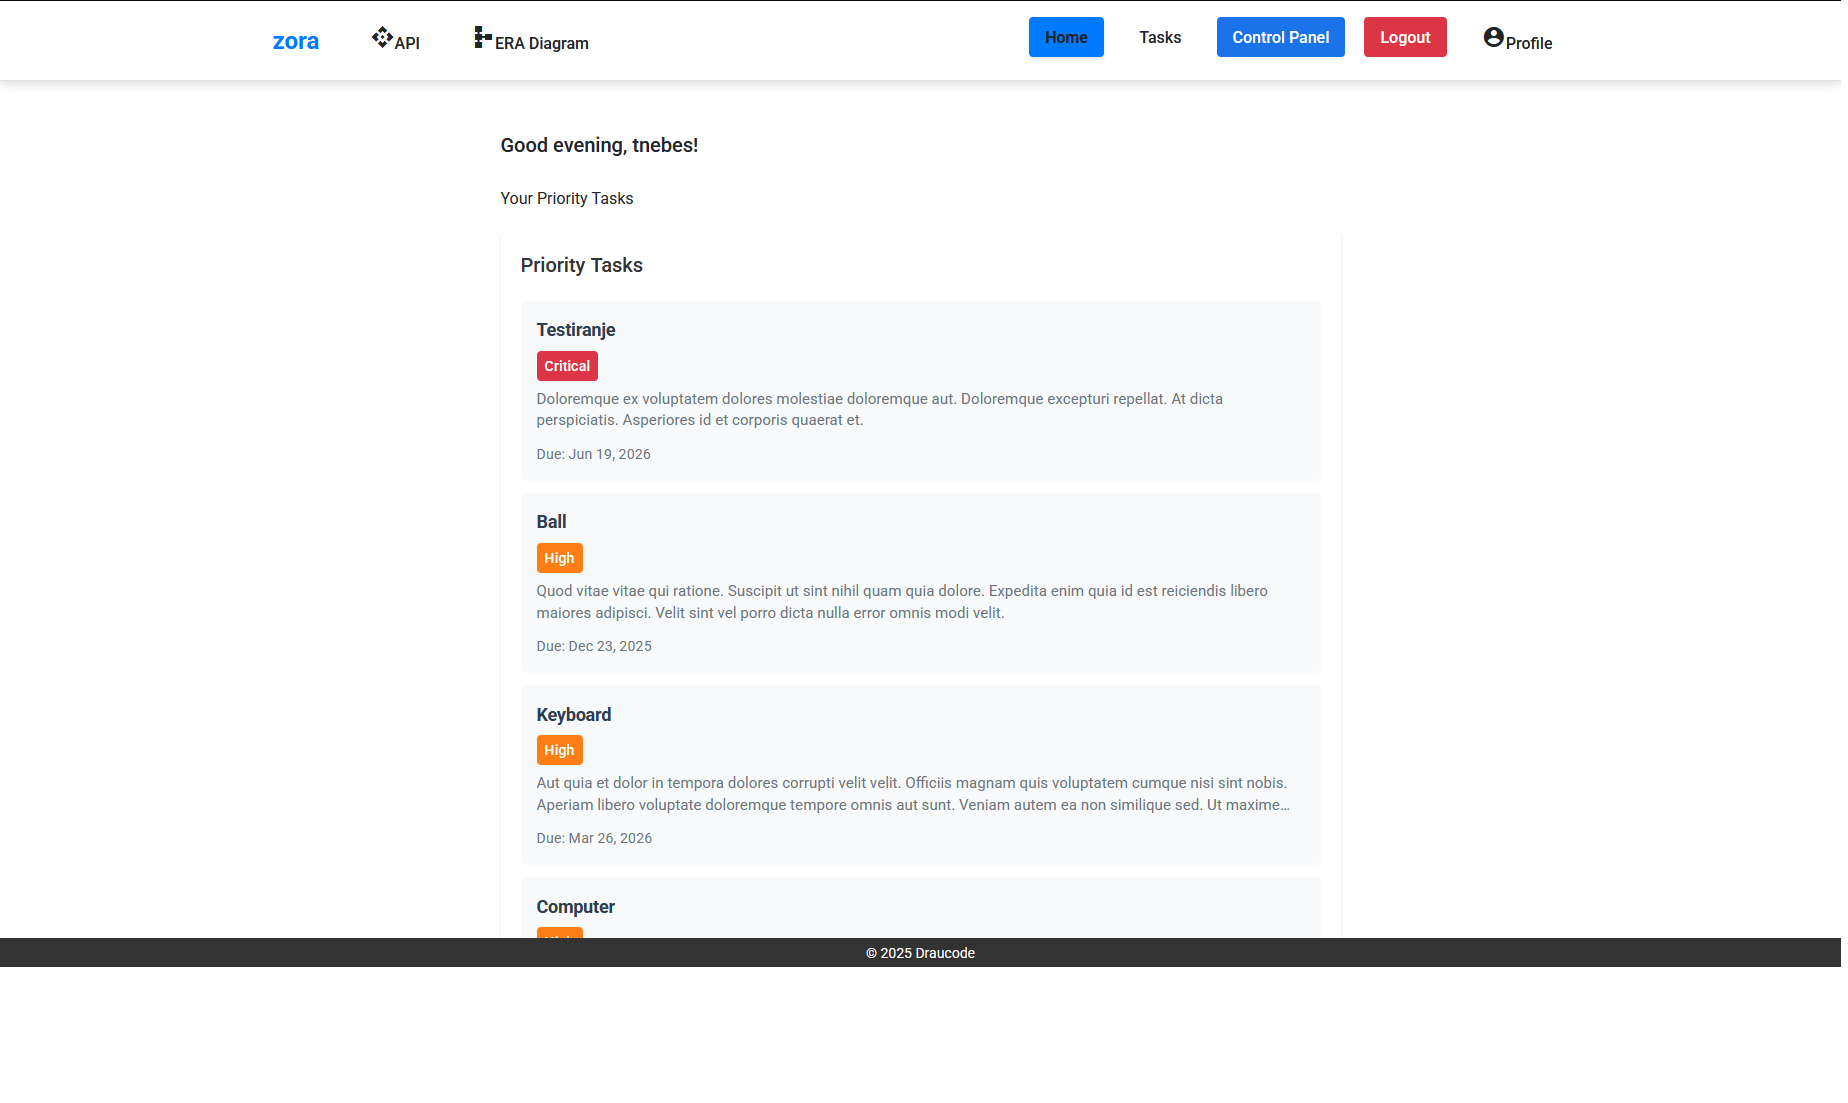
\includegraphics[width=\textwidth]{frontend_example.png}
\end{center}

\end{document}
